\chapter{Desarrollo} % Título del capítulo

\label{Desarrollo}

\section{Selección del microcontrolador}

\label{Selec}

Resulta imprescindible que el microcontrolador seleccionado para este proyecto de investigación cumpla con los siguientes requisitos:

%cambiar-listo!
\begin{itemize}
    \item Estar basado en una ISA RISC-V, ya que el contexto del proyecto está orientado a acoplar coprocesadores en núcleos RISC-V.
    \item Estar descrito en el lenguaje de descripción de hardware VHDL, ya que los coprocesadores embebidos para aplicaciones de IA que se pretenden acoplar están descritos en este lenguaje.
    \item Contar con extensión de instrucciones para conectar coprocesadores mediante CFU, además de con soporte para comunicaciones \textit{memory-mapped} e interfaces \textit{stream}, ya que se necesita una variedad de métodos de conexión para realizar la caracterización del rendimiento mediante diferentes modos.
\end{itemize} 

En este sentido, el NEORV32 \cite{gh:neorv32} cumple con todos estos requerimientos. 
Además, en la plataforma de desarrollo colaborativo donde está alojado, cuenta con una comunidad muy activa.
Es por ello que se encuentra bajo una revisión constante de \textit{bugs} (fallos), tanto por parte del autor como de los usuarios.
De esta manera, se asegura en gran medida la correcta operatividad del mismo.
Además, el autor se dedica a realizar actualizaciones periódicas de sus funcionalidades.
Por si fuera poco, tanto el autor como la comunidad tienen una gran disponibilidad para responder dudas sobre temas relacionados con el proyecto, lo que resulta de gran ayuda.
Con respecto a la compilación de lenguajes de alto nivel, el proyecto ofrece \textit{toolchains} precompiladas de RISC-V para GCC.  
Estas herramientas permiten hacer compilación cruzada de C/C++ a instrucciones de RISC-V  en un entorno Linux \cite{gh:neorv32-tool}.
Cabe destacar que también se facilita un contenedor para realizar esta tarea \cite{gh:sim-conatiner}. 
Además, cuenta con un soporte de librerías para compilar funciones software específicas de NEORV32. 
Asimismo, el repositorio ofrece una variedad de ejemplos de aplicación software de todos los recursos con los que cuenta el micro.
En adición a todo lo mencionado, este microcontrolador cuenta con un \textit{datasheet} \cite{neorv32-ds} y una \textit{user guide} \cite{neorv32-ug} realizadas por el autor y actualizadas a la par que el código del proyecto, las cuales destacan por su calidad.
Teniendo en cuenta todas estas consideraciones, el NEORV32 es el procesador seleccionado para este proyecto.

\hspace{10 mm}

\section{\textit{Workflow}}

\label{Workf}

Las herramientas EDA FLOS y las propietarias/comerciales no son ecosistemas aislados.
Al contrario, en los últimos años se han visto colaboraciones de proyectos \textit{Open Source} con iniciativas privativas.
En este sentido, se puede destacar la integración de la herramienta RapidWright \cite{gh:rapid} a la \textit{Suite} de diseño Vivado.
En concreto, este proyeto \textit{Open Source} desarrollado por \textit{AMD Research and Advanced Development} tiene como objetivo permitir a los usuarios avanzados una mayor flexibilidad a la hora de personalizar sus soluciones mediante una metodología de diseño utilizando módulos pre-implementados.
En adición a esto, se han realizado concursos \cite{contest} patrocinados por AMD con el objetivo de promover y demostrar que el \textit{FPGA Interchange Format} (FPGAIF - Formato de Intercambio de FPGA) \cite{FPGAIF} es una representación intermediaria eficiente y robusta para trabajar en problemas de \textit{backends} de FPGAs, incluso a escala industrial.
Además, este tipo de iniciativas también tratan de fomentar la innovación de algoritmos de enrutamiento de FPGAs que den prioridad al tiempo de ejecución, con objeto de posibilitar su aplicación en la emulación de ASICs.
Cabe destacar que el FPGAIF es un estándar de formato de intercambio diseñado para proporcionar toda la información necesaria mediante la cual realizar el \textit{place and route} en un contexto \textit{Open Source}.
En la misma línea, Siemens ha observado un crecimiento saludable entorno a la \textit{Open Source VHDL Verification Methodology} (OSVVM - Metodología de Verificación VHDL de Código Abierto) \cite{osvvm} y la \textit{Universal VHDL Verification Methodology} (UVVM -  Metodología de Verificación Universal VHDL) \cite{uvvm} desde 2018, lo que en sus propias palabras \say{es alentador} \cite{wilson-research}.
Por lo tanto, a la vista de estos ejemplos, podemos afirmar que los comerciales tradicionales de herramientas EDA están empezando a facilitar el uso de herramientas FLOS e incluso a integrar parte o la totalidad de las mismas en sus propuestas comerciales.
Este hecho refleja un futuro híbrido en lo referente al ecosistema de herramientas para FPGAs.

\begin{figure}[h!]
    \centering
    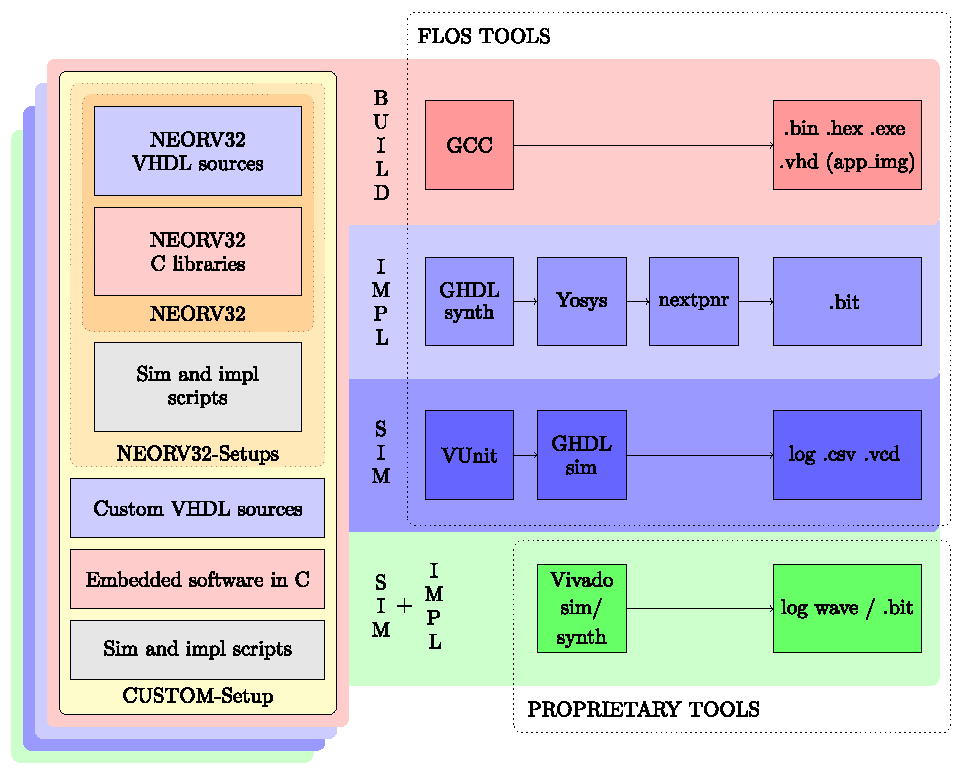
\includegraphics[width=14cm]{Figuras/workflow.pdf}
    \caption{\textit{Workflow} del \textit{Setup} personalizado.}
    \label{fig:workf}
\end{figure}

Atendiendo a este nuevo paradigma híbrido de herramientas, en el presente trabajo de investigación se propone el uso tanto de herramientas FLOS como privativas.
Como se observa en la figura \ref{fig:workf}, el flujo de trabajo propuesto es el siguiente:

\begin{itemize}
    \item Compilación: respecto a la compilación de software en C que posteriormente se cargará en la memoria de instrucciones del NEORV32, se emplea exclusivamente la herramienta FLOS GCC.
    \item Implementación: respecto a las implementaciones en placa de los diseños, se efectúan todas ellas tanto para la Arty A7 35T como para la Arty A7 100T y mediante dos vías paralelas:
        \begin{itemize}
            \item Haciendo uso del conjunto de herramientas FLOS: GHDL \cite{gh:ghdl}, yosys \cite{gh:yosys}, GHDL yosys plugin \cite{gh:ghdl-plugin}, nextpnr-xilinx \cite{gh:nextpnr} y prjxray \cite{gh:prjxray} para realizar la elaboración, la síntesis y el \textit{place and route} y de la herramienta openFPGALoader \cite{gh:openFPGALoader} para cargar el \textit{bitstream} en la placa.
            \item Haciendo uso de la \textit{Suite} de diseño privativa Vivado.
        \end{itemize}
    \item Simulación: respecto a las simulaciones realizadas a lo largo de las secciones \ref{Carac} y \ref{Integ} se emplea principalmente el \textit{framework} FLOS VUnit \cite{gh:vunit}, con el cual se realizan todas ellas.
No obstante, también se utiliza Vivado en ciertas ocasiones.  
En concreto, en los ensayos en los que se hace uso de la funcionalidad ILA.
Esta funcionalidad se ha utilizado, por ejemplo, para testear la correcta operatividad de un \textit{wrapper} Wishbone.
\end{itemize} 

El conjunto de herramientas descritas en la explicación de este flujo de trabajo no solo se utilizan a nivel local, también se utilizan, todas o parte de ellas, en \textbf{integración continua (CI)} en repositorios \textit{online}, tanto en el GitLab del grupo de investigación como en el GitHub propio.
Para ello, se utilizan varios \textbf{contenedores}.
Para la generación de \textit{bitstream} mediante herramientas FLOS, se utiliza el contenedor mencionado en la sección \ref{ben}, el cual es generado a su vez en CI.
Este contenedor se utiliza en la integración continua tanto del repositorio ubicado en GitLab como del ubicado en GitHub.
Para la generación de \textit{bitstream} mediante Vivado, se utiliza una contenedor que solamente es accesible por los ordenadores del laboratorio del grupo de investigación, el cual está alojado en nuestro servidor Orion.
Esto es debido a que al ser un software privativo el contenedor no puede ser accesible sin licencia, es por ello que la generación de \textit{bitstream} mediante esta vía solo está disponible en la integración continua del repositorio del grupo (GitLab).
Para realizar los ensayos en simulación, se utilizan principalmente dos contenedores de VUnit.
El \href{https://console.cloud.google.com/gcr/images/hdl-containers/global/sim/osvb}{gcr.io/hdl-containers/sim/osvb:latest} con GHDL compilado con llvm como \textit{backend} y el \href{https://hub.docker.com/layers/ghdl/vunit/mcode-master/images/sha256-e32029c5be70a5fa0fc94bffd15d72fa8b84ad8aaf2dc7cfa8ab8324ef733ed0?context=explore}{docker.io/ghdl/vunit:mcode-master} con GHDL compilado con mcode como \textit{backend}.
Esto se debe a que la funcionalidad \href{https://github.com/stnolting/neorv32/discussions/886}{\textit{external names}}, para capturar señales de jerarquías inferiores, solo es soportada en GHDL si este está compilado con el \textit{backend} mcode.
En definitiva, haciendo uso de estos contenedores mediante la metodología de integración continua, se consigue generar de forma automatizada los resultados de todas las simulaciones, así como la generación de todos los \textit{bitstreams}, cada vez que se hace un \textit{push} al repositorio.
Cabe destacar que la compilación de software solo se realiza en local, aunque también se utiliza un contenedor \cite{gh:sim-conatiner}, no está automatizada en integración continua.

\subsection{Cargar software en el NEORV32}

Antes de entrar en los detalles del acoplamiento de periféricos \textit{custom}, se procede a realizar un repaso de como cargar un software en C al \textit{softcore} NEORV32.
Como se ha mencionado, el proyecto NEORV32 proporciona herramientas para realizar la compilación cruzada desde Linux a la arquitectura RISC-V.
Estas herramientas están acompañadas de archivos \textit{Makefiles} mediante los cuales se permiten añadir argumentos al comando \textit{Make}, con objeto de, entre otras cosas, proporcionar el programa compilado en diferentes formatos de salida.
A lo largo de esta sección, nos centraremos en tres de estos formatos:

\begin{itemize}
    \item Ejecutable, \textit{exe} (.bin)
    \item app\_image (.vhd)
    \item Hexadecimal (.hex)
\end{itemize} 

Cada una de estas salidas tiene la misma información, el programa compilado.
No obstante, cada una de ellas puede utilizarse para cargar el software en la IMEM (memoria de instrucciones) en diferentes puntos del \textit{Workflow}:

\begin{itemize}
    \item El \textit{exe} se puede cargar en el NEORV32 una vez que esté ejecutándose en la FPGA. Esta transferencia se realiza a través del \textit{bootloader}.
    \item La app\_image remplaza el contenido por defecto de una de las fuentes RTL del diseño del NEORV32, de modo que su contenido se codifica cuando este se sintetiza.
    \item El archivo .hex se lee durante la síntesis, por lo que es equivalente a la solución de la app\_image, pero no requiere modificar las fuentes RTL cada vez que se actualiza el software a cargar.
\end{itemize} 

Estas opciones se resumen en la siguiente tabla:

\begin{table}[h!]
\centering
\caption{Tres formas de introducir software en la IMEM.}
\label{tab:2}
\begin{tabular}{|c|c|c|c|}
\hline
\textbf{Formato}  & \textbf{Comando}   & \textbf{Descripción}                                                                                            & \textbf{Bootloader}  \\ \hline
.bin              & make exe           & \begin{tabular}[c]{@{}c@{}}Después de la implementación,\\  cargar el exe mediante la CMD\end{tabular}          & Habilitado           \\ \hline
.vhd              & make image         & \begin{tabular}[c]{@{}c@{}}Antes de la síntesis, \\ sustituir la app\_image por defecto\end{tabular}            & Deshabilitado        \\ \hline
.hex              & make hex           & Durante la síntesis, leer del .hex                                                                              & Deshabilitado        \\ \hline
\end{tabular}
\end{table}

\subsubsection{\textit{Bootloader}}
\label{boot}

El NEORV32 viene por defecto con un \textit{bootloader} que se encarga de establecer la comunicación serie vía UART y generar una CMD visible desde terminales como CuteCom \cite{gh:cutecom}, \href{https://man.openbsd.org/cu.1}{cu}, o \href{https://www.gnu.org/software/screen/}{screen} en GNU/Linux.
En este sentido, hay tres formas posibles de proceder:

\begin{itemize}
    \item Deshabilitar el \textit{bootloader} y cargar/iniciar un programa desde la app\_image o desde un archivo hexadecimal.
        \begin{itemize}
            \item No se utiliza el \textit{bootloader}.
        \end{itemize} 
    \item Habilitar el \textit{bootloader} y cargar/iniciar un programa a través del \textit{Autoboot}.
        \begin{itemize}
            \item Después del \textit{reset}, cuando el \textit{bootloader} está habilitado, la primera secuencia que ocurre es el \textit{Autoboot}.
            \item La secuencia de \textit{Autoboot} intenta obtener una imagen de arranque válida desde la flash SPI externa.
            \item Si se encuentra una imagen de arranque válida que se pueda transferir correctamente a la IMEM (memoria de instrucciones), se inicia automáticamente la aplicación.
            \item Si han pasado 8 segundos y no se ha detectado ninguna flash SPI o no se encuentra ninguna imagen de arranque válida, se mostrará el código de error \say{ERR EXE}, bloqueando la ejecución del \textit{bootloader}.
            \item Durante esos 8 segundos, se puede detener la secuencia del \textit{Autoboot} pulsando cualquier tecla. 
De esta manera, se pone a disposición una CMD lista para recibir comandos.
        \end{itemize} 
    \item Habilitar el \textit{bootloader} y cargar/iniciar un programa a través de comandos en la CMD.
Los comandos soportados son los siguientes:
        \begin{itemize}
            \item \say{h} - Muestra el texto de ayuda.
            \item \say{r} - Reiniciar el \textit{bootloader}.
            \item \say{u} - Cargar un programa en formato ejecutable (\textit{neorv32\_exe.bin}) a la IMEM.
            \item \say{s} - Almacenar un ejecutable en flash SPI.
            \item \say{l} - Cargar un ejecutable desde flash SPI.
            \item \say{x} - Arrancar un programa desde flash a través de XIP.
            \item \say{e} - Iniciar un programa almacenado en la IMEM.
        \end{itemize} 
\end{itemize} 

Para elegir una de estas tres formas de proceder, se debe entender que el \textit{bootloader} es útil/necesario cuando:

    \begin{itemize}
        \item La FPGA utilizada no permite inicializar la memoria en el \textit{bitstream}. 
En consecuencia, no es posible cargar/arrancar programas a través de la app\_image.
Este es el caso de las FPGAs con SPRAM, como la Lattice ICE40 (UP3K, UP5K).
        \item Múltiples programas deben ser cargados/arrancados durante el desarrollo, sin resintetizar el diseño.
    \end{itemize} 

En la figura \ref{fig:boot} se muestra como cargar/iniciar un programa ejecutable (.exe) al NEORV32 mediante el \textit{bootloader}. 
Concretamente, en ese caso se utiliza la terminal CuteCom \footnote {En CuteCom, el archivo que se carga a la terminal debe ser de tipo \textit{Plain} (como se muestra en la figura \ref{fig:boot}), de lo contrario se dará el error \say{ERR EXE}.}, empleando sucesivamente los comandos \say{u} (\textit{upload} - cargar) y \say{e} (\textit{execute} - ejecutar).

\begin{figure}[h!]
    \centering
    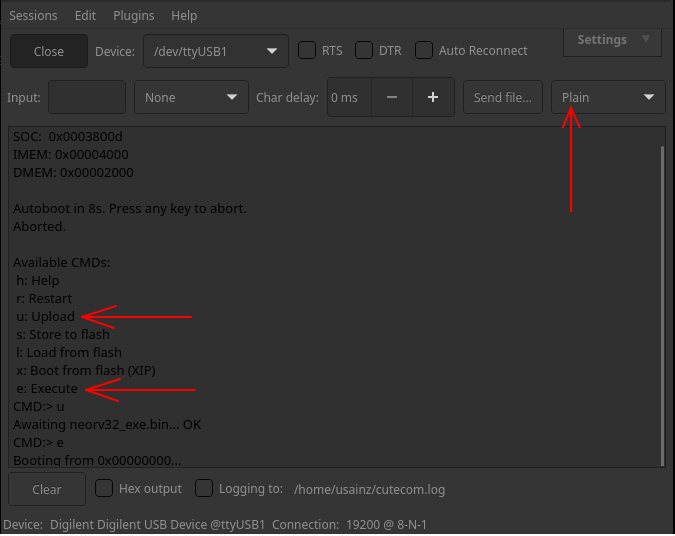
\includegraphics[width=14cm]{Figuras/cutecom_cmd_upload.png}
    \caption{Cargar un \textit{exe} a través del \textit{bootloader} de NEORV32 (terminal CuteCom).}
    \label{fig:boot}
\end{figure}


\subsubsection{Habilitar/Deshabilitar el \textit{Bootloader}}

Si el \textit{bootloader} no es útil/necesario para nuestra aplicación tendremos que considerar lo siguiente.
La IMEM se puede implementar de dos formas, como una RAM vacía o como una ROM inicializada a través del archivo que contiene el programa compilado, ya sea la \textit{neorv32\_application\_image.vhd} o el hexadecimal. 
Con el genérico \mintinline[breaklines]{vhdl}{IMEM_AS_IROM} se selecciona la implementación de la IMEM mediante una de estas dos opciones. 
Este genérico es
 
\hspace{35mm} {\mintinline[breaklines]{vhdl}{IMEM_AS_IROM => imem_as_rom_c} }

\noindent y se define como 

\hspace{17mm} \mintinline[breaklines]{vhdl}{imem_as_rom_c : boolean := not INT_BOOTLOADER_EN;}

\noindent Por lo tanto, para cargar un programa desde la \textit{neorv32\_application\_image.vhd} (o desde el hexadecimal), la IMEM debe implementarse como una ROM inicializada mediante ese archivo, por lo que el \textit{bootloader} \textbf{debe estar deshabilitado}.
Se discutió con Stephan \href{https://github.com/stnolting/neorv32/discussions/824}{(\#824)} acerca de por qué la IMEM se inicializa como una RAM vacía cuando el \textit{bootloader} está activado. 
Y según el diseñador del NEORV32, \say{si la IMEM se implementara como una RAM preinicializada, entonces la imagen podría corromperse durante el tiempo de ejecución (imagina algún puntero deshonesto escribiendo en la IMEM), lo que requeriría volver a cargar el programa original. 
Por lo tanto, la carga del \textit{bootloader} se requeriría de todos modos.}

El proceso para deshabilitar el \textit{bootloader} es sencillo, en el TOP del diseño del NEORV32, se debe cambiar la constante \mintinline[breaklines]{vhdl}{INT_BOOTLOADER_EN} de \textit{true} a \textit{false}, como se muestra en el extracto de código \ref{code:1}.

\begin{listing}[h!]
\begin{minted}[frame=lines,framesep=2mm,baselinestretch=1.2,fontsize=\footnotesize]{vhdl}
neorv32_top_inst : neorv32_top
generic map(
----------------------------------
INT_BOOTLOADER_EN         => false,
----------------------------------
)
\end{minted}
\caption{Constante para deshabilitar el \textit{bootloader}.}
\label{code:1}
\end{listing}

\subsubsection{Cargar un programa compilado desde un archivo hexadecimal}

Como se ha mencionado, en vez de cargar un programa compilado desde el archivo \textit{neorv32\_application\_image.vhd}, es posible cargar el programa compilado desde un archivo hexadecimal (.hex).
Para ello, se necesitan hacer unas pequeñas modificaciones en el código HDL del NEORV32.
En particular, se debe añadir una nueva función en el paquete \textit{neorve32\_package.vhd}.
Esta función se encargará de leer el archivo hexadecimal usando la librería \textit{std.textio.all}. \footnote{Esta librería está soportada desde la versión VHDL 2008.}
La función en cuestión es la descrita en el extracto de código \ref{code:2}.

\begin{listing}[h!]
\begin{minted}[frame=lines,framesep=2mm,baselinestretch=1.2,fontsize=\footnotesize]{vhdl}
-- Initialize mem32_t from hex
-- MEMORY_SIZE is IMEM_SIZE/4, see neorv32_imem.default.vhd

impure function mem32_init_hex(name : STRING; MEMORY_SIZE : natural) return mem32_t is
    file rom_file : text open read_mode is name;
    variable rom_line : line;
    variable temp_word : std_ulogic_vector(31 downto 0);
    variable temp_rom : mem32_t(0 to MEMORY_SIZE-1) := (others => (others => '0'));
begin
    for i in 0 to MEMORY_SIZE - 1 loop
        exit when endfile(rom_file);
        readline(rom_file, rom_line);
        hread(rom_line, temp_word);
        temp_rom(i) := temp_word;
    end loop;

    return temp_rom;
end function;
\end{minted}
\caption{Función a añadir al \textit{neorve32\_package.vhd} para leer un software compilado en formato hexadecimal.}
\label{code:2}
\end{listing}

Además, el archivo \textit{neorv32\_imem.default.vhd} \footnote{En el archivo \textit{neorv32\_imem.default.vhd} el código relacionado con cargar la ROM desde la app\_image debe ser comentado.} se debe modificar para cargar el contenido del archivo hexadecimal a la memoria de instrucciones, usando la función definida en el extracto de código \ref{code:2}.
Para ello se debe añadir el extracto de código \ref{code:3}.

\begin{listing}[h!]
\begin{minted}[frame=lines,framesep=2mm,baselinestretch=1.2,fontsize=\footnotesize]{vhdl}
constant ROM_INIT_FILE : string := "neorv32_raw_exe.hex";
-- ROM - initialized with hex code --
constant mem_rom_c : mem32_t(0 to IMEM_SIZE/4-1) := mem32_init_hex(ROM_INIT_FILE, IMEM_SIZE/4);
\end{minted}
\caption{Modificación del archivo \textit{neorv32\_imem.default.vhd} para cargar la IMEM mediante la función descrita en el extracto de código \ref{code:2}.}
\label{code:3}
\end{listing}

En conclusión, este método propone leer desde un formato hexadecimal, el cual es una salida nativa del compilador, 
a través de código VHDL, en lugar de autogenerar código HDL con el programa compilado. 
Ambas opciones cargan la IMEM cuando se sintetiza el diseño, pero la opción de lectura del archivo .hex no modifica el código HDL del diseño. 
Es decir, con esta opción conseguimos dos cosas, no autogenerar código en otro lenguaje y no modificar el código HDL cada vez que se actualiza el software a cargar.

Por último, cabe destacar que a lo largo del desarrollo de este proyecto se ha cargado software compilado al NEORV32 mediante los tres formatos expuestos.
No obstante, mayoritariamente se ha utilizado el formato .vhd generando una \textit{neorv32   \_application\_image.vhd} para cada software empleado.

\section{Caracterización del rendimiento}

\label{Carac}

\section{Integración de coprocesador para aplicaciones de IA}

\label{Integ}


